% Created by tikzDevice version 0.12.3.1 on 2023-03-27 19:44:12
% !TEX encoding = UTF-8 Unicode
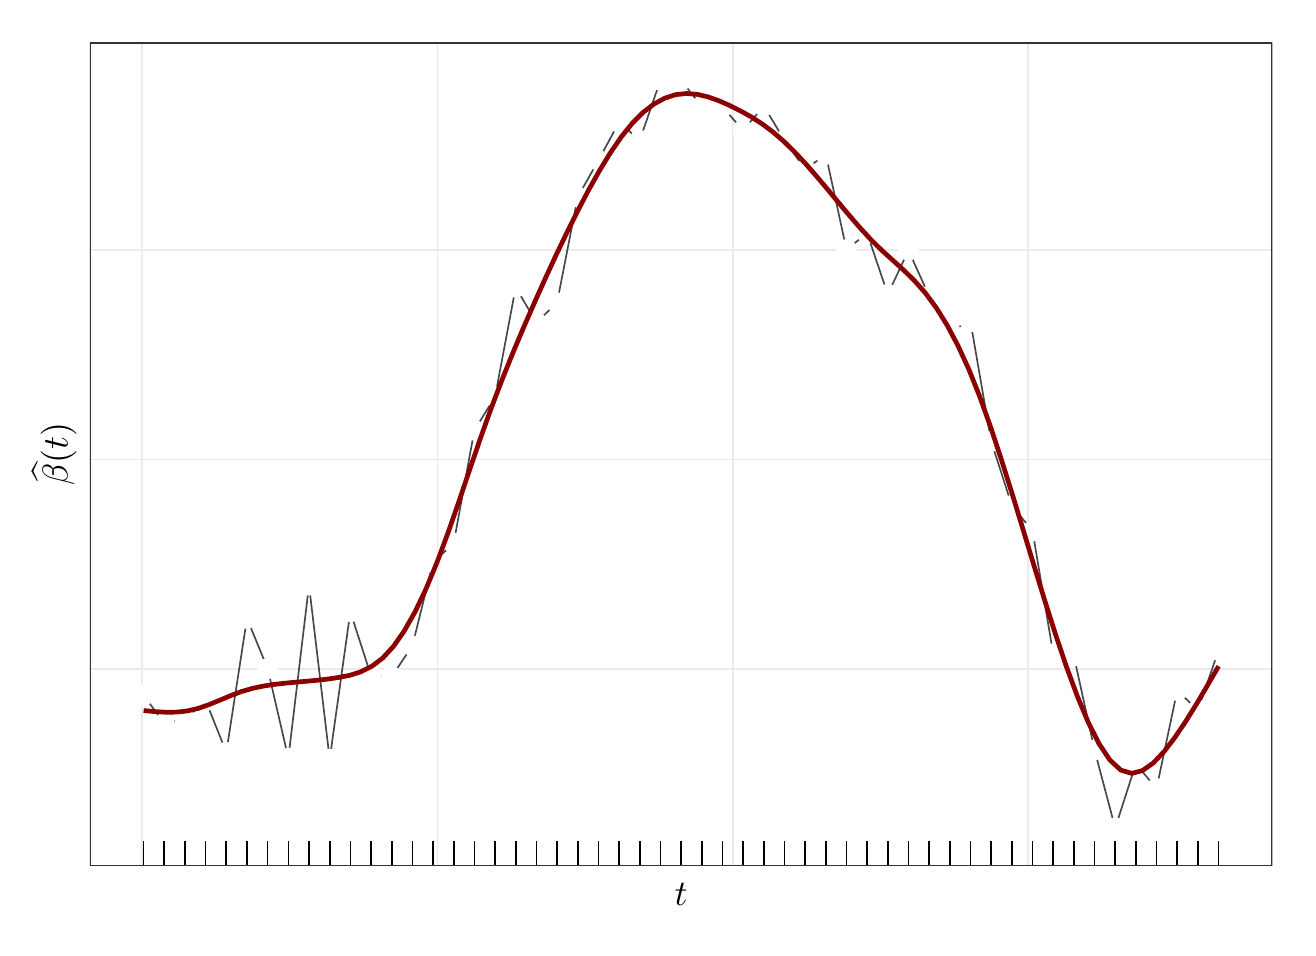
\begin{tikzpicture}[x=1pt,y=1pt]
\definecolor{fillColor}{RGB}{255,255,255}
\path[use as bounding box,fill=fillColor,fill opacity=0.00] (0,0) rectangle (455.24,325.17);
\begin{scope}
\path[clip] (  0.00,  0.00) rectangle (455.24,325.17);
\definecolor{drawColor}{RGB}{255,255,255}
\definecolor{fillColor}{RGB}{255,255,255}

\path[draw=drawColor,line width= 0.6pt,line join=round,line cap=round,fill=fillColor] (  0.00,  0.00) rectangle (455.24,325.17);
\end{scope}
\begin{scope}
\path[clip] ( 22.48, 22.48) rectangle (449.74,319.67);
\definecolor{fillColor}{RGB}{255,255,255}

\path[fill=fillColor] ( 22.48, 22.48) rectangle (449.74,319.67);
\definecolor{drawColor}{gray}{0.92}

\path[draw=drawColor,line width= 0.6pt,line join=round] ( 22.48, 93.42) --
	(449.74, 93.42);

\path[draw=drawColor,line width= 0.6pt,line join=round] ( 22.48,169.11) --
	(449.74,169.11);

\path[draw=drawColor,line width= 0.6pt,line join=round] ( 22.48,244.80) --
	(449.74,244.80);

\path[draw=drawColor,line width= 0.6pt,line join=round] ( 41.37, 22.48) --
	( 41.37,319.67);

\path[draw=drawColor,line width= 0.6pt,line join=round] (148.08, 22.48) --
	(148.08,319.67);

\path[draw=drawColor,line width= 0.6pt,line join=round] (254.79, 22.48) --
	(254.79,319.67);

\path[draw=drawColor,line width= 0.6pt,line join=round] (361.49, 22.48) --
	(361.49,319.67);
\definecolor{drawColor}{RGB}{0,0,0}

\path[draw=drawColor,line width= 0.6pt,line join=round] ( 41.90, 22.48) -- ( 41.90, 31.40);

\path[draw=drawColor,line width= 0.6pt,line join=round] ( 49.37, 22.48) -- ( 49.37, 31.40);

\path[draw=drawColor,line width= 0.6pt,line join=round] ( 56.84, 22.48) -- ( 56.84, 31.40);

\path[draw=drawColor,line width= 0.6pt,line join=round] ( 64.31, 22.48) -- ( 64.31, 31.40);

\path[draw=drawColor,line width= 0.6pt,line join=round] ( 71.78, 22.48) -- ( 71.78, 31.40);

\path[draw=drawColor,line width= 0.6pt,line join=round] ( 79.25, 22.48) -- ( 79.25, 31.40);

\path[draw=drawColor,line width= 0.6pt,line join=round] ( 86.72, 22.48) -- ( 86.72, 31.40);

\path[draw=drawColor,line width= 0.6pt,line join=round] ( 94.19, 22.48) -- ( 94.19, 31.40);

\path[draw=drawColor,line width= 0.6pt,line join=round] (101.66, 22.48) -- (101.66, 31.40);

\path[draw=drawColor,line width= 0.6pt,line join=round] (109.13, 22.48) -- (109.13, 31.40);

\path[draw=drawColor,line width= 0.6pt,line join=round] (116.60, 22.48) -- (116.60, 31.40);

\path[draw=drawColor,line width= 0.6pt,line join=round] (124.07, 22.48) -- (124.07, 31.40);

\path[draw=drawColor,line width= 0.6pt,line join=round] (131.54, 22.48) -- (131.54, 31.40);

\path[draw=drawColor,line width= 0.6pt,line join=round] (139.01, 22.48) -- (139.01, 31.40);

\path[draw=drawColor,line width= 0.6pt,line join=round] (146.48, 22.48) -- (146.48, 31.40);

\path[draw=drawColor,line width= 0.6pt,line join=round] (153.95, 22.48) -- (153.95, 31.40);

\path[draw=drawColor,line width= 0.6pt,line join=round] (161.42, 22.48) -- (161.42, 31.40);

\path[draw=drawColor,line width= 0.6pt,line join=round] (168.89, 22.48) -- (168.89, 31.40);

\path[draw=drawColor,line width= 0.6pt,line join=round] (176.35, 22.48) -- (176.35, 31.40);

\path[draw=drawColor,line width= 0.6pt,line join=round] (183.82, 22.48) -- (183.82, 31.40);

\path[draw=drawColor,line width= 0.6pt,line join=round] (191.29, 22.48) -- (191.29, 31.40);

\path[draw=drawColor,line width= 0.6pt,line join=round] (198.76, 22.48) -- (198.76, 31.40);

\path[draw=drawColor,line width= 0.6pt,line join=round] (206.23, 22.48) -- (206.23, 31.40);

\path[draw=drawColor,line width= 0.6pt,line join=round] (213.70, 22.48) -- (213.70, 31.40);

\path[draw=drawColor,line width= 0.6pt,line join=round] (221.17, 22.48) -- (221.17, 31.40);

\path[draw=drawColor,line width= 0.6pt,line join=round] (228.64, 22.48) -- (228.64, 31.40);

\path[draw=drawColor,line width= 0.6pt,line join=round] (236.11, 22.48) -- (236.11, 31.40);

\path[draw=drawColor,line width= 0.6pt,line join=round] (243.58, 22.48) -- (243.58, 31.40);

\path[draw=drawColor,line width= 0.6pt,line join=round] (251.05, 22.48) -- (251.05, 31.40);

\path[draw=drawColor,line width= 0.6pt,line join=round] (258.52, 22.48) -- (258.52, 31.40);

\path[draw=drawColor,line width= 0.6pt,line join=round] (265.99, 22.48) -- (265.99, 31.40);

\path[draw=drawColor,line width= 0.6pt,line join=round] (273.46, 22.48) -- (273.46, 31.40);

\path[draw=drawColor,line width= 0.6pt,line join=round] (280.93, 22.48) -- (280.93, 31.40);

\path[draw=drawColor,line width= 0.6pt,line join=round] (288.40, 22.48) -- (288.40, 31.40);

\path[draw=drawColor,line width= 0.6pt,line join=round] (295.87, 22.48) -- (295.87, 31.40);

\path[draw=drawColor,line width= 0.6pt,line join=round] (303.34, 22.48) -- (303.34, 31.40);

\path[draw=drawColor,line width= 0.6pt,line join=round] (310.81, 22.48) -- (310.81, 31.40);

\path[draw=drawColor,line width= 0.6pt,line join=round] (318.28, 22.48) -- (318.28, 31.40);

\path[draw=drawColor,line width= 0.6pt,line join=round] (325.75, 22.48) -- (325.75, 31.40);

\path[draw=drawColor,line width= 0.6pt,line join=round] (333.22, 22.48) -- (333.22, 31.40);

\path[draw=drawColor,line width= 0.6pt,line join=round] (340.69, 22.48) -- (340.69, 31.40);

\path[draw=drawColor,line width= 0.6pt,line join=round] (348.16, 22.48) -- (348.16, 31.40);

\path[draw=drawColor,line width= 0.6pt,line join=round] (355.63, 22.48) -- (355.63, 31.40);

\path[draw=drawColor,line width= 0.6pt,line join=round] (363.10, 22.48) -- (363.10, 31.40);

\path[draw=drawColor,line width= 0.6pt,line join=round] (370.57, 22.48) -- (370.57, 31.40);

\path[draw=drawColor,line width= 0.6pt,line join=round] (378.03, 22.48) -- (378.03, 31.40);

\path[draw=drawColor,line width= 0.6pt,line join=round] (385.50, 22.48) -- (385.50, 31.40);

\path[draw=drawColor,line width= 0.6pt,line join=round] (392.97, 22.48) -- (392.97, 31.40);

\path[draw=drawColor,line width= 0.6pt,line join=round] (400.44, 22.48) -- (400.44, 31.40);

\path[draw=drawColor,line width= 0.6pt,line join=round] (407.91, 22.48) -- (407.91, 31.40);

\path[draw=drawColor,line width= 0.6pt,line join=round] (415.38, 22.48) -- (415.38, 31.40);

\path[draw=drawColor,line width= 0.6pt,line join=round] (422.85, 22.48) -- (422.85, 31.40);

\path[draw=drawColor,line width= 0.6pt,line join=round] (430.32, 22.48) -- (430.32, 31.40);
\definecolor{drawColor}{RGB}{10,10,10}

\path[draw=drawColor,draw opacity=0.75,line width= 0.6pt,line join=round] ( 41.90, 83.90) --
	( 49.37, 73.80) --
	( 56.84, 75.33) --
	( 64.31, 82.01) --
	( 71.78, 63.32) --
	( 79.25,111.72) --
	( 86.72, 93.54) --
	( 94.19, 61.19) --
	(101.66,123.72) --
	(109.13, 60.85) --
	(116.60,114.12) --
	(124.07, 90.94) --
	(131.54, 90.70) --
	(139.01,101.81) --
	(146.48,131.89) --
	(153.95,138.91) --
	(161.42,179.70) --
	(168.89,191.82) --
	(176.35,231.36) --
	(183.82,218.61) --
	(191.29,225.79) --
	(198.76,263.99) --
	(206.23,277.22) --
	(213.70,291.00) --
	(221.17,284.48) --
	(228.64,306.16) --
	(236.11,306.10) --
	(243.58,296.73) --
	(251.05,296.48) --
	(258.52,288.11) --
	(265.99,296.82) --
	(273.46,284.51) --
	(280.93,273.97) --
	(288.40,279.33) --
	(295.87,245.00) --
	(303.34,250.84) --
	(310.81,228.82) --
	(318.28,244.74) --
	(325.75,228.11) --
	(333.22,215.62) --
	(340.69,218.89) --
	(348.16,175.71) --
	(355.63,152.50) --
	(363.10,143.27) --
	(370.57, 98.97) --
	(378.03, 98.14) --
	(385.50, 64.21) --
	(392.97, 35.99) --
	(400.44, 59.14) --
	(407.91, 50.23) --
	(415.38, 85.61) --
	(422.85, 78.61) --
	(430.32,100.11);
\definecolor{drawColor}{RGB}{255,255,255}

\path[draw=drawColor,line width= 0.4pt,line join=round,line cap=round,fill=fillColor] ( 41.90, 83.90) circle (  3.57);

\path[draw=drawColor,line width= 0.4pt,line join=round,line cap=round,fill=fillColor] ( 49.37, 73.80) circle (  3.57);

\path[draw=drawColor,line width= 0.4pt,line join=round,line cap=round,fill=fillColor] ( 56.84, 75.33) circle (  3.57);

\path[draw=drawColor,line width= 0.4pt,line join=round,line cap=round,fill=fillColor] ( 64.31, 82.01) circle (  3.57);

\path[draw=drawColor,line width= 0.4pt,line join=round,line cap=round,fill=fillColor] ( 71.78, 63.32) circle (  3.57);

\path[draw=drawColor,line width= 0.4pt,line join=round,line cap=round,fill=fillColor] ( 79.25,111.72) circle (  3.57);

\path[draw=drawColor,line width= 0.4pt,line join=round,line cap=round,fill=fillColor] ( 86.72, 93.54) circle (  3.57);

\path[draw=drawColor,line width= 0.4pt,line join=round,line cap=round,fill=fillColor] ( 94.19, 61.19) circle (  3.57);

\path[draw=drawColor,line width= 0.4pt,line join=round,line cap=round,fill=fillColor] (101.66,123.72) circle (  3.57);

\path[draw=drawColor,line width= 0.4pt,line join=round,line cap=round,fill=fillColor] (109.13, 60.85) circle (  3.57);

\path[draw=drawColor,line width= 0.4pt,line join=round,line cap=round,fill=fillColor] (116.60,114.12) circle (  3.57);

\path[draw=drawColor,line width= 0.4pt,line join=round,line cap=round,fill=fillColor] (124.07, 90.94) circle (  3.57);

\path[draw=drawColor,line width= 0.4pt,line join=round,line cap=round,fill=fillColor] (131.54, 90.70) circle (  3.57);

\path[draw=drawColor,line width= 0.4pt,line join=round,line cap=round,fill=fillColor] (139.01,101.81) circle (  3.57);

\path[draw=drawColor,line width= 0.4pt,line join=round,line cap=round,fill=fillColor] (146.48,131.89) circle (  3.57);

\path[draw=drawColor,line width= 0.4pt,line join=round,line cap=round,fill=fillColor] (153.95,138.91) circle (  3.57);

\path[draw=drawColor,line width= 0.4pt,line join=round,line cap=round,fill=fillColor] (161.42,179.70) circle (  3.57);

\path[draw=drawColor,line width= 0.4pt,line join=round,line cap=round,fill=fillColor] (168.89,191.82) circle (  3.57);

\path[draw=drawColor,line width= 0.4pt,line join=round,line cap=round,fill=fillColor] (176.35,231.36) circle (  3.57);

\path[draw=drawColor,line width= 0.4pt,line join=round,line cap=round,fill=fillColor] (183.82,218.61) circle (  3.57);

\path[draw=drawColor,line width= 0.4pt,line join=round,line cap=round,fill=fillColor] (191.29,225.79) circle (  3.57);

\path[draw=drawColor,line width= 0.4pt,line join=round,line cap=round,fill=fillColor] (198.76,263.99) circle (  3.57);

\path[draw=drawColor,line width= 0.4pt,line join=round,line cap=round,fill=fillColor] (206.23,277.22) circle (  3.57);

\path[draw=drawColor,line width= 0.4pt,line join=round,line cap=round,fill=fillColor] (213.70,291.00) circle (  3.57);

\path[draw=drawColor,line width= 0.4pt,line join=round,line cap=round,fill=fillColor] (221.17,284.48) circle (  3.57);

\path[draw=drawColor,line width= 0.4pt,line join=round,line cap=round,fill=fillColor] (228.64,306.16) circle (  3.57);

\path[draw=drawColor,line width= 0.4pt,line join=round,line cap=round,fill=fillColor] (236.11,306.10) circle (  3.57);

\path[draw=drawColor,line width= 0.4pt,line join=round,line cap=round,fill=fillColor] (243.58,296.73) circle (  3.57);

\path[draw=drawColor,line width= 0.4pt,line join=round,line cap=round,fill=fillColor] (251.05,296.48) circle (  3.57);

\path[draw=drawColor,line width= 0.4pt,line join=round,line cap=round,fill=fillColor] (258.52,288.11) circle (  3.57);

\path[draw=drawColor,line width= 0.4pt,line join=round,line cap=round,fill=fillColor] (265.99,296.82) circle (  3.57);

\path[draw=drawColor,line width= 0.4pt,line join=round,line cap=round,fill=fillColor] (273.46,284.51) circle (  3.57);

\path[draw=drawColor,line width= 0.4pt,line join=round,line cap=round,fill=fillColor] (280.93,273.97) circle (  3.57);

\path[draw=drawColor,line width= 0.4pt,line join=round,line cap=round,fill=fillColor] (288.40,279.33) circle (  3.57);

\path[draw=drawColor,line width= 0.4pt,line join=round,line cap=round,fill=fillColor] (295.87,245.00) circle (  3.57);

\path[draw=drawColor,line width= 0.4pt,line join=round,line cap=round,fill=fillColor] (303.34,250.84) circle (  3.57);

\path[draw=drawColor,line width= 0.4pt,line join=round,line cap=round,fill=fillColor] (310.81,228.82) circle (  3.57);

\path[draw=drawColor,line width= 0.4pt,line join=round,line cap=round,fill=fillColor] (318.28,244.74) circle (  3.57);

\path[draw=drawColor,line width= 0.4pt,line join=round,line cap=round,fill=fillColor] (325.75,228.11) circle (  3.57);

\path[draw=drawColor,line width= 0.4pt,line join=round,line cap=round,fill=fillColor] (333.22,215.62) circle (  3.57);

\path[draw=drawColor,line width= 0.4pt,line join=round,line cap=round,fill=fillColor] (340.69,218.89) circle (  3.57);

\path[draw=drawColor,line width= 0.4pt,line join=round,line cap=round,fill=fillColor] (348.16,175.71) circle (  3.57);

\path[draw=drawColor,line width= 0.4pt,line join=round,line cap=round,fill=fillColor] (355.63,152.50) circle (  3.57);

\path[draw=drawColor,line width= 0.4pt,line join=round,line cap=round,fill=fillColor] (363.10,143.27) circle (  3.57);

\path[draw=drawColor,line width= 0.4pt,line join=round,line cap=round,fill=fillColor] (370.57, 98.97) circle (  3.57);

\path[draw=drawColor,line width= 0.4pt,line join=round,line cap=round,fill=fillColor] (378.03, 98.14) circle (  3.57);

\path[draw=drawColor,line width= 0.4pt,line join=round,line cap=round,fill=fillColor] (385.50, 64.21) circle (  3.57);

\path[draw=drawColor,line width= 0.4pt,line join=round,line cap=round,fill=fillColor] (392.97, 35.99) circle (  3.57);

\path[draw=drawColor,line width= 0.4pt,line join=round,line cap=round,fill=fillColor] (400.44, 59.14) circle (  3.57);

\path[draw=drawColor,line width= 0.4pt,line join=round,line cap=round,fill=fillColor] (407.91, 50.23) circle (  3.57);

\path[draw=drawColor,line width= 0.4pt,line join=round,line cap=round,fill=fillColor] (415.38, 85.61) circle (  3.57);

\path[draw=drawColor,line width= 0.4pt,line join=round,line cap=round,fill=fillColor] (422.85, 78.61) circle (  3.57);

\path[draw=drawColor,line width= 0.4pt,line join=round,line cap=round,fill=fillColor] (430.32,100.11) circle (  3.57);
\definecolor{drawColor}{RGB}{139,0,0}

\path[draw=drawColor,line width= 1.7pt,line join=round] ( 41.90, 78.41) --
	( 45.83, 78.04) --
	( 49.75, 77.81) --
	( 53.67, 77.84) --
	( 57.60, 78.25) --
	( 61.52, 79.16) --
	( 65.44, 80.52) --
	( 69.37, 82.13) --
	( 73.29, 83.78) --
	( 77.21, 85.26) --
	( 81.14, 86.40) --
	( 85.06, 87.24) --
	( 88.98, 87.84) --
	( 92.91, 88.29) --
	( 96.83, 88.66) --
	(100.75, 89.00) --
	(104.68, 89.36) --
	(108.60, 89.81) --
	(112.52, 90.38) --
	(116.45, 91.16) --
	(120.37, 92.40) --
	(124.29, 94.36) --
	(128.22, 97.32) --
	(132.14,101.55) --
	(136.06,107.16) --
	(139.99,114.10) --
	(143.91,122.31) --
	(147.83,131.74) --
	(151.76,142.27) --
	(155.68,153.53) --
	(159.60,165.11) --
	(163.53,176.59) --
	(167.45,187.55) --
	(171.38,197.85) --
	(175.30,207.59) --
	(179.22,216.89) --
	(183.15,225.86) --
	(187.07,234.61) --
	(190.99,243.10) --
	(194.92,251.29) --
	(198.84,259.15) --
	(202.76,266.62) --
	(206.69,273.62) --
	(210.61,280.03) --
	(214.53,285.73) --
	(218.46,290.61) --
	(222.38,294.55) --
	(226.30,297.57) --
	(230.23,299.70) --
	(234.15,300.96) --
	(238.07,301.38) --
	(242.00,301.06) --
	(245.92,300.13) --
	(249.84,298.73) --
	(253.77,297.00) --
	(257.69,295.04) --
	(261.61,292.83) --
	(265.54,290.29) --
	(269.46,287.34) --
	(273.38,283.94) --
	(277.31,280.08) --
	(281.23,275.85) --
	(285.15,271.36) --
	(289.08,266.70) --
	(293.00,261.97) --
	(296.93,257.28) --
	(300.85,252.75) --
	(304.77,248.50) --
	(308.70,244.65) --
	(312.62,241.10) --
	(316.54,237.55) --
	(320.47,233.71) --
	(324.39,229.27) --
	(328.31,223.96) --
	(332.24,217.65) --
	(336.16,210.26) --
	(340.08,201.71) --
	(344.01,191.90) --
	(347.93,180.94) --
	(351.85,169.08) --
	(355.78,156.59) --
	(359.70,143.75) --
	(363.62,130.82) --
	(367.55,118.06) --
	(371.47,105.75) --
	(375.39, 94.14) --
	(379.32, 83.51) --
	(383.24, 74.14) --
	(387.16, 66.36) --
	(391.09, 60.49) --
	(395.01, 56.88) --
	(398.93, 55.71) --
	(402.86, 56.72) --
	(406.78, 59.51) --
	(410.70, 63.67) --
	(414.63, 68.81) --
	(418.55, 74.65) --
	(422.48, 80.98) --
	(426.40, 87.64) --
	(430.32, 94.42);
\definecolor{drawColor}{RGB}{0,0,0}

\node[text=drawColor,anchor=base,inner sep=0pt, outer sep=0pt, scale=  1.10] at ( 41.90, 80.10) {$\upbeta$};

\node[text=drawColor,anchor=base,inner sep=0pt, outer sep=0pt, scale=  1.10] at ( 49.37, 70.00) {$\upbeta$};

\node[text=drawColor,anchor=base,inner sep=0pt, outer sep=0pt, scale=  1.10] at ( 56.84, 71.53) {$\upbeta$};

\node[text=drawColor,anchor=base,inner sep=0pt, outer sep=0pt, scale=  1.10] at ( 64.31, 78.21) {$\upbeta$};

\node[text=drawColor,anchor=base,inner sep=0pt, outer sep=0pt, scale=  1.10] at ( 71.78, 59.52) {$\upbeta$};

\node[text=drawColor,anchor=base,inner sep=0pt, outer sep=0pt, scale=  1.10] at ( 79.25,107.92) {$\upbeta$};

\node[text=drawColor,anchor=base,inner sep=0pt, outer sep=0pt, scale=  1.10] at ( 86.72, 89.74) {$\upbeta$};

\node[text=drawColor,anchor=base,inner sep=0pt, outer sep=0pt, scale=  1.10] at ( 94.19, 57.39) {$\upbeta$};

\node[text=drawColor,anchor=base,inner sep=0pt, outer sep=0pt, scale=  1.10] at (101.66,119.92) {$\upbeta$};

\node[text=drawColor,anchor=base,inner sep=0pt, outer sep=0pt, scale=  1.10] at (109.13, 57.05) {$\upbeta$};

\node[text=drawColor,anchor=base,inner sep=0pt, outer sep=0pt, scale=  1.10] at (116.60,110.31) {$\upbeta$};

\node[text=drawColor,anchor=base,inner sep=0pt, outer sep=0pt, scale=  1.10] at (124.07, 87.14) {$\upbeta$};

\node[text=drawColor,anchor=base,inner sep=0pt, outer sep=0pt, scale=  1.10] at (131.54, 86.89) {$\upbeta$};

\node[text=drawColor,anchor=base,inner sep=0pt, outer sep=0pt, scale=  1.10] at (139.01, 98.01) {$\upbeta$};

\node[text=drawColor,anchor=base,inner sep=0pt, outer sep=0pt, scale=  1.10] at (146.48,128.08) {$\upbeta$};

\node[text=drawColor,anchor=base,inner sep=0pt, outer sep=0pt, scale=  1.10] at (153.95,135.11) {$\upbeta$};

\node[text=drawColor,anchor=base,inner sep=0pt, outer sep=0pt, scale=  1.10] at (161.42,175.90) {$\upbeta$};

\node[text=drawColor,anchor=base,inner sep=0pt, outer sep=0pt, scale=  1.10] at (168.89,188.02) {$\upbeta$};

\node[text=drawColor,anchor=base,inner sep=0pt, outer sep=0pt, scale=  1.10] at (176.35,227.56) {$\upbeta$};

\node[text=drawColor,anchor=base,inner sep=0pt, outer sep=0pt, scale=  1.10] at (183.82,214.81) {$\upbeta$};

\node[text=drawColor,anchor=base,inner sep=0pt, outer sep=0pt, scale=  1.10] at (191.29,221.99) {$\upbeta$};

\node[text=drawColor,anchor=base,inner sep=0pt, outer sep=0pt, scale=  1.10] at (198.76,260.19) {$\upbeta$};

\node[text=drawColor,anchor=base,inner sep=0pt, outer sep=0pt, scale=  1.10] at (206.23,273.41) {$\upbeta$};

\node[text=drawColor,anchor=base,inner sep=0pt, outer sep=0pt, scale=  1.10] at (213.70,287.20) {$\upbeta$};

\node[text=drawColor,anchor=base,inner sep=0pt, outer sep=0pt, scale=  1.10] at (221.17,280.68) {$\upbeta$};

\node[text=drawColor,anchor=base,inner sep=0pt, outer sep=0pt, scale=  1.10] at (228.64,302.36) {$\upbeta$};

\node[text=drawColor,anchor=base,inner sep=0pt, outer sep=0pt, scale=  1.10] at (236.11,302.30) {$\upbeta$};

\node[text=drawColor,anchor=base,inner sep=0pt, outer sep=0pt, scale=  1.10] at (243.58,292.93) {$\upbeta$};

\node[text=drawColor,anchor=base,inner sep=0pt, outer sep=0pt, scale=  1.10] at (251.05,292.68) {$\upbeta$};

\node[text=drawColor,anchor=base,inner sep=0pt, outer sep=0pt, scale=  1.10] at (258.52,284.31) {$\upbeta$};

\node[text=drawColor,anchor=base,inner sep=0pt, outer sep=0pt, scale=  1.10] at (265.99,293.01) {$\upbeta$};

\node[text=drawColor,anchor=base,inner sep=0pt, outer sep=0pt, scale=  1.10] at (273.46,280.71) {$\upbeta$};

\node[text=drawColor,anchor=base,inner sep=0pt, outer sep=0pt, scale=  1.10] at (280.93,270.17) {$\upbeta$};

\node[text=drawColor,anchor=base,inner sep=0pt, outer sep=0pt, scale=  1.10] at (288.40,275.53) {$\upbeta$};

\node[text=drawColor,anchor=base,inner sep=0pt, outer sep=0pt, scale=  1.10] at (295.87,241.19) {$\upbeta$};

\node[text=drawColor,anchor=base,inner sep=0pt, outer sep=0pt, scale=  1.10] at (303.34,247.04) {$\upbeta$};

\node[text=drawColor,anchor=base,inner sep=0pt, outer sep=0pt, scale=  1.10] at (310.81,225.02) {$\upbeta$};

\node[text=drawColor,anchor=base,inner sep=0pt, outer sep=0pt, scale=  1.10] at (318.28,240.93) {$\upbeta$};

\node[text=drawColor,anchor=base,inner sep=0pt, outer sep=0pt, scale=  1.10] at (325.75,224.31) {$\upbeta$};

\node[text=drawColor,anchor=base,inner sep=0pt, outer sep=0pt, scale=  1.10] at (333.22,211.82) {$\upbeta$};

\node[text=drawColor,anchor=base,inner sep=0pt, outer sep=0pt, scale=  1.10] at (340.69,215.09) {$\upbeta$};

\node[text=drawColor,anchor=base,inner sep=0pt, outer sep=0pt, scale=  1.10] at (348.16,171.90) {$\upbeta$};

\node[text=drawColor,anchor=base,inner sep=0pt, outer sep=0pt, scale=  1.10] at (355.63,148.70) {$\upbeta$};

\node[text=drawColor,anchor=base,inner sep=0pt, outer sep=0pt, scale=  1.10] at (363.10,139.47) {$\upbeta$};

\node[text=drawColor,anchor=base,inner sep=0pt, outer sep=0pt, scale=  1.10] at (370.57, 95.17) {$\upbeta$};

\node[text=drawColor,anchor=base,inner sep=0pt, outer sep=0pt, scale=  1.10] at (378.03, 94.33) {$\upbeta$};

\node[text=drawColor,anchor=base,inner sep=0pt, outer sep=0pt, scale=  1.10] at (385.50, 60.41) {$\upbeta$};

\node[text=drawColor,anchor=base,inner sep=0pt, outer sep=0pt, scale=  1.10] at (392.97, 32.19) {$\upbeta$};

\node[text=drawColor,anchor=base,inner sep=0pt, outer sep=0pt, scale=  1.10] at (400.44, 55.33) {$\upbeta$};

\node[text=drawColor,anchor=base,inner sep=0pt, outer sep=0pt, scale=  1.10] at (407.91, 46.43) {$\upbeta$};

\node[text=drawColor,anchor=base,inner sep=0pt, outer sep=0pt, scale=  1.10] at (415.38, 81.81) {$\upbeta$};

\node[text=drawColor,anchor=base,inner sep=0pt, outer sep=0pt, scale=  1.10] at (422.85, 74.81) {$\upbeta$};

\node[text=drawColor,anchor=base,inner sep=0pt, outer sep=0pt, scale=  1.10] at (430.32, 96.31) {$\upbeta$};
\definecolor{drawColor}{gray}{0.20}

\path[draw=drawColor,line width= 0.6pt,line join=round,line cap=round] ( 22.48, 22.48) rectangle (449.74,319.67);
\end{scope}
\begin{scope}
\path[clip] (  0.00,  0.00) rectangle (455.24,325.17);
\definecolor{drawColor}{RGB}{0,0,0}

\node[text=drawColor,anchor=base,inner sep=0pt, outer sep=0pt, scale=  1.30] at (236.11,  8.03) {$t$};
\end{scope}
\begin{scope}
\path[clip] (  0.00,  0.00) rectangle (455.24,325.17);
\definecolor{drawColor}{RGB}{0,0,0}

\node[text=drawColor,rotate= 90.00,anchor=base,inner sep=0pt, outer sep=0pt, scale=  1.30] at ( 14.45,171.08) {$\widehat{\beta} (t)$};
\end{scope}
\end{tikzpicture}
